
%%%%%%%%%%%%%%%%%%%%%%% file typeinst.tex %%%%%%%%%%%%%%%%%%%%%%%%%
%
% This is the LaTeX source for the instructions to authors using
% the LaTeX document class 'llncs.cls' for contributions to
% the Lecture Notes in Computer Sciences series.
% http://www.springer.com/lncs       Springer Heidelberg 2006/05/04
%
% It may be used as a template for your own input - copy it
% to a new file with a new name and use it as the basis
% for your article.
%
% NB: the document class 'llncs' has its own and detailed documentation, see
% ftp://ftp.springer.de/data/pubftp/pub/tex/latex/llncs/latex2e/llncsdoc.pdf
%
%%%%%%%%%%%%%%%%%%%%%%%%%%%%%%%%%%%%%%%%%%%%%%%%%%%%%%%%%%%%%%%%%%%


\documentclass[runningheads,a4paper]{llncs}

\usepackage{amssymb}
\setcounter{tocdepth}{3}
\usepackage{graphicx}
\usepackage{subfig}
\usepackage{cite}
\usepackage{multicol}
%\usepackage{subcaption}

\usepackage{url}
\urldef{\mailsa}\path|Logan.C.Farrell@NASA.gov, Troy.A.Dennis@rice.edu|    
\newcommand{\keywords}[1]{\par\addvspace\baselineskip
\noindent\keywordname\enspace\ignorespaces#1}

\begin{document}

\mainmatter  % start of an individual contribution

% first the title is needed
\title{Simply Grasping Simple Shapes:\\
Commanding a Humanoid Hand with a Shape-Based Synergy}

% a short form should be given in case it is too long for the running head
\titlerunning{Simply Grasping Simple Shapes}

% the name(s) of the author(s) follow(s) next
%
% NB: Chinese authors should write their first names(s) in front of
% their surnames. This ensures that the names appear correctly in
% the running heads and the author index.
%
\author{Logan C. Farrell$^{1,2}$ %
\and Troy A. Dennis$^{1}$\and Julia Badger$^{2}$\and Marcia K. O'Malley$^{1}$}
%
\authorrunning{Simply Grasping Simple Shapes}
% (feature abused for this document to repeat the title also on left hand pages)

% the affiliations are given next; don't give your e-mail address
% unless you accept that it will be published
\institute{$^{1}$Mechanical Engineering, Rice University, Houston, USA\\$^{2}$Johnson Space Center, NASA, Houston, USA}


%
% NB: a more complex sample for affiliations and the mapping to the
% corresponding authors can be found in the file "llncs.dem"
% (search for the string "\mainmatter" where a contribution starts).
% "llncs.dem" accompanies the document class "llncs.cls".
%

\toctitle{Lecture Notes in Computer Science}
\tocauthor{Authors' Instructions}
\maketitle


\begin{abstract}
Despite rapid advancements in dexterity and mechanical design, the utility of humanoid robots in an uncontrolled laboratory setting is limited in part due to the complexity involved in programming robots to grasp common objects. There exists a need for an efficient method to command high degree-of-freedom (DoF) , position-controlled, dexterous manipulators for a range of objects such that explicit models are not needed for every interaction. The authors propose a method incorporating the neuroscience concept of postural synergies to decrease the commanded DoFs to match intuitive measurements of an object to be grasped, which we term geometrical synergies.  The approach of this paper is similar to that of Ciocarlie et al. \cite{ciocarlieallen}, however, rather than testing the postural synergies that come from the principle components of a human grasps, the authors design a grasping synergy based on the object that is meant to be grasped by the robot.  For this paper, a synergy was designed to grasp cylinder-shaped objects. Using the SynGrasp toolbox, a model of Robonaut 2`s twelve-DoF hand was created to perform contact analysis around a small set of cylinders defined by a single variable, diameter. Experiments were performed on the robot to validate and update the synergy-based models.  Successful manipulation of a large range of cylindrical objects, not previously introduced to the robot, was demonstrated in a proof-of-concept experiment. This synergy-based grasp planning method can be applied to any position-controlled humanoid hand to decrease the number of commanded DoF based on simple, measureable inputs. to grasp commonly shaped objects. This method has the potential to vastly multiply the library of objects the robot can manipulate.
\keywords{Manipulation, Grasp, Synergy, Humanoid, Dexterous Hand}
\end{abstract}


\section{Introduction}

Humanoid robots provide the capability to operate in the same space, using the same tools that a human can. The future of these robots can clearly be seen with efforts for robots to go into disaster areas unsafe for humans \cite{fukushima_robots} or help humans do menial tasks. Perhaps the most fundamental capability necessary to accomplish these human tasks is the ability to manipulate the same objects that humans can. For this challenge, many designers have created hands capable of nearly all of the DoFs as the human hand \cite{r2_hand}, \cite{DRL}, \cite{hrp3}, \cite{softhand}. However, while the hands are able to form many of the same grips and poses as a human hand, the control of these hands in an intuitive and simple way has yet to be demonstrated. Until the community can quickly and effectively control these high DoF humanoid hands, robots will still need to be highly specialized for individual tasks. \par
Research shows that humans control their hands not with individual joint position commands, as dexterous robot hands are typically controlled, but instead by a single signal that actuates multiple muscle groups. These groups combine to create the plethora of hand motions humans can form \cite{Santello} \cite{neuro}. This approach gives a method for decreasing the commanded DoF of the hand system to a more manageable number, and is referred to as ``synergies". These synergy schemes represent the principle components of various grasps of the human hand. These components can be difficult to intuitively combine into useful hand motions, shifting the complexity problem from DoF, to nonintuitive combinations of synergies. \par
The contribution of this paper is a methodology to decrease the commanded DoF from twelve to one for the Robonaut 2 (R2) hand to manipulate simple cylindrical shapes. This methodology replaces all unique cylindrical type models with a single model to allow simple manipulation of common objects. In addition, the single commanded DoF is based on a simple measurement of the object to allow intuitive control. This enables the robot to successfully manipulate any cylindrical object found in its environment with the single model.

\section{Background}


\subsection{Hand Synergies}
	Dexterous manipulation in robots has developed from a simple parallel gripper towards the complexity of the human hand in the past decades. These devices are high DoF systems that allow robots to manipulate objects in similar ways to a human. However, as this problem has been studied further, the construction of robotic hands with similar DoFs as the human hand has become common place, but the control is anything but intuitive. The computational costs to calculate the correct closing position around a given object as perceived by a robotic vision system is $O(2^N)$
 where N represents the number of DoFs, with each DoF controlled individually. Researchers have focused on analyzing the way that humans control our own hands with hopes of extending that same control scheme to a robotic hand, as in the seminal work on postural synergies of human grasping \cite{Santello}. 

Neurological studies have demonstrated that the human brain does not plan and execute specific movements of the individual finger joints. Instead, our brain will send high level commands down through the motor cortex to execute sets of actions, and these commands will travel down the spine to activate sets of muscles in combination, rather than just single muscle groups. In this way, our brain is grouping and combining sets of commands in different ways to accomplish the task \cite{neuro}.  Santello et al. performed Principal Component Analysis (PCA) on a large range of everyday grasps, and was able to model 50$\%$ of the variability in the grasps with a single relationship, or synergy. If a second synergy was added in proportion, roughly 80$\%$  of the variability in grasps could be commanded. Similarly the third synergy resulted in modeling 90$\%$  of observed grasp variability. This coupling demonstrates how our brain is potentially reducing the 20 DoF problem of hand motion into only a few DoFs. Thinking in this way greatly reduces the complexity of grasping for humans and allows smooth control of a very large number of DoFs to accomplish grasping  tasks without a large burden on the nervous system. 

 Engineers can draw inspiration from this structure to design robotic grasping devices.  A synergistic scheme can be implemented in several ways.  Human hand synergies can be used to identify key DoFs that are necessary for a simplified hand design.  They can also be used to devise under-actuation schemes such as the PISA-IIT soft-hand \cite{softhand}.  Finally, they can be used to simplify the control of fully actuated hands by creating ``Software Synergies" \cite{catalano_2012_adaptive}.  

 One of these Software Synergies was demonstrated by Ciorcarlie et al. \cite{ciocarlie_2007_dexterous}.  The group used the GraspIt software to map the two primary human postural synergies to fully actuated robotic hands.  Roa et al. \cite{power_grasp} used a more involved algorithm to study the contacts on complex objects by partitioning the object into planar slices, studying form and force closure  \cite{bicchi} to determine optimal hand closure. An interesting aspect of this approach was it calculated the optimal thumb and index finger closure, and then calculated the remaining fingers to stabilize the grasp.   Garcia et. al. demonstrated how human synergy based motion planning can be used to decrease the computation time for motion planning in humanoid dual arm robot system  \cite{garcia}.

SynGrasp, a MATLAB toolbox developed for the purpose of simulating underactuated robot grasping, is another computational tool based on synergies \cite{syngrasp}.  This toolbox offers three primary capabilities: it allows the user to model robotic hands, perform grasp simulations and analysis, and map synergies on to robot hand designs. SynGrasp is well suited to designing and testing  synergy schemes using kinematics \cite{salvietti_2016_map}.  We also aim to create our own unique purpose-driven synergy scheme instead of attempting to replicate human postural synergies.

The ability to create user-defined hand models and synergies makes SynGrasp an ideal tool for simulating a synergy based command structure on R2.  A computational tool for modeling grasps and commands would be hugely beneficial for evaluation of the hand and for designing grips for it. %replace this sentence
While the main purpose of this study is to evaluate a synergy command architecture, it will have the added objective of evaluating the use and accuracy of SynGrasp simulations in real-world environments.

\subsection{Test Platform and Motivation}

NASA is actively developing humanoid robotics to work in the same environment as astronauts. To this end, Robonaut 2 is a humanoid robot with two 7 DoF arms (including the wrist), a 3 DoF neck, 1 DoF waist, two 12 DoF hands, and two 7 DoF legs. R2 is currently on board the International Space Station (see Fig \ref{at_r2_iss}. The design goal of this robot is to assist astronauts with repetitive tasks on the International Space Station like monitoring airflow, cleaning handrails, and unpacking resupply vehicles \cite{r2_diftler}. Currently, NASA is actively developing technologies to allow this robot to behave with more autonomy. This is necessary to allow supervised control over long time delays as missions progress farther and farther from Earth. 

   \begin{figure}[t]
      \centering
      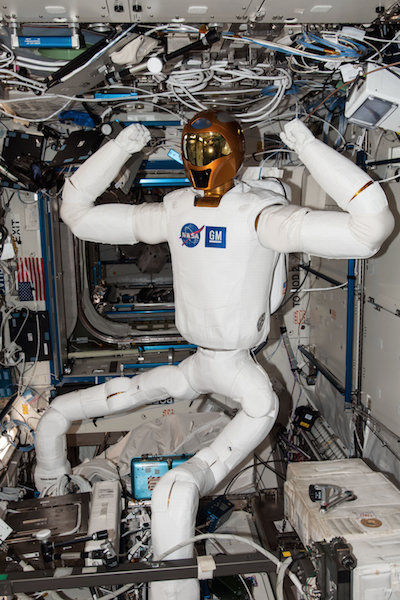
\includegraphics[width=0.4\textwidth]{r2_iss}
      \caption{Robonaut 2 aboard the International Space Station}
      \label{at_r2_iss}
   \end{figure}

To achieve this level of autonomy and dexterity, it becomes intractible to set specific values for each robot joint to form every possible hand pose that R2 might require on board the ISS. Currently, each object to be manipulated must be modeled, the approach trajectories defined and tested, and the necessary hand positions specified and verified. However, if the complexity of commands to control grasps can be decreased from 12 DoF to 1 DoF, this task becomes significantly simpler. Instead of modeling and planning grasps for each individual object, a single shape-based model could be developed and verified. Then, the robot will have a model to manipulate any similarly shaped object encountered. The application of synergies in this case will save time and effort while increasing the capability and usefulness of the dexterous robot.   


\subsection{Current Implementation of R2 Pose and Object Feature Based Grasping}
R2's command structure centers around the concept of multi-loop control with a series of embedded loops \cite{r2_control}. The lowest level of control is a current loop, wrapped by a velocity loop, wrapped by a torque loop, and finally wrapped by a position loop that specified the desired finger poses. 
Because the actuators that position R2's fingers are not series-elastic and have no direct torque measurement capability, the control structure of the R2 hand is modified compared to that used for the series elastic joints in the arms and legs. The torque control loop is removed and current limiting is added to the lowest control loop to protect the finger tendons. Without hte capability of direct torque control of the finger joints, the fingers can only be position controlled. For R2 to grasp complex-shaped objects, precise models of object geometry and accurate position control are required. Thus, the postural-syngery based grasp control schemes that have seen success in control of compliant robot hands \cite{} will be ineffective for control of R2. 

   \begin{figure}[!b]
      \centering
      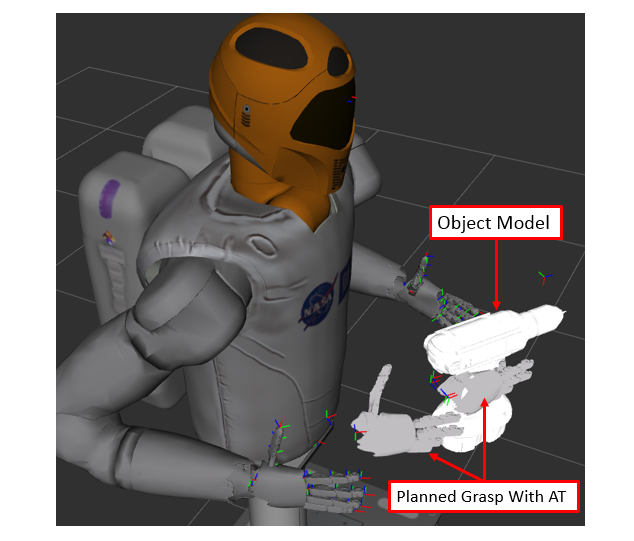
\includegraphics[width=0.6\textwidth]{drill_at2}
      \caption{Robonaut 2 current method for manipulation of a drill using the Affordance Template (AT).  This approach requires a CAD model of the object to be grasped and multiple inputs (grasp position, grasp type) from the user}
      \label{at_example}
   \end{figure}

Given the necessity to accurately command finger-joint positions in the R2 hand to achieve grasping, the original grasp process used by R2 was based on the Cutkosky Grasp Taxonomy \cite{Cutkosky}. This series of 24 position defined grasps composed the main method of grasping an object. For full manipulation, the Cutkosky grasps are used in conjunction with the Affordance Template Framework \cite{affordance_templates} that builds manipulation models for objects to be grasped, similar to systems used for other humanoid robots \cite{DRC_Yanco}, \cite{IHMC}. 
This approach results in unique pairings of a single object affordance template with an appropriate Cutkosky grasp. An example affordance template is shown in Fig \ref{at_example}. To grasp the object differently, a new grasp must be created, tested, and verified. To grasp a new object, even if it differs only slightly from the orignial, the entire affordance template creation process must be repeated. 

This repeated creation of templates and grasp positions can be time consuming and application specific, and is intractable at a large scale for robots in practice. Further, the method of using pose-based synergies of the human hand are equally non-intuitive to implement in a position control based scheme. A new approach is needed, one that allows for determination of robot hand positions based on simple geometric poerperties of the object to be grasped. In this paper, the authors propose a geometric synergy based on cylindrical type objects. The finger position can be commanded based on a single variable dictated by the object, it's diameter. This would allow a objects such as a flash light, a coffee cup, a screwdriver, and any other cylinder to be manipulated using the same cylindrical template based solely on the objects diameter. 

\section{Methods}

\label{methods}

% take this section from 3 paragraphs down to 3 sentences. We basically say all of this somewhere else. 
A synergistic command structure can be mathematically defined in (1).
$$
q = S\sigma  \eqno{(1)}
$$
where $q$ is the vector of joint angles of dimensions [$N \times 1$],  $N$ is the number of synergies, $S$ is the synergy matrix of dimensions [$N \times M$],  $M$ is the number of possible synergies that can be activated and $\sigma$ is the [$M \times 1$] synergy activation vector which determines which synergy or combination thereof is turned on.  The basis of synergies is that the generic joint displacement, $q$, can be represented as a function of fewer elements than the number of DoFs of the system.  $S$ is a vector of weights that determines the amount of motion for an individual joint resulting from a single input.  In neuroscience, these $S$ matrices are determined by mapping the grasps of various shapes and isolating the movements of individual joints.  The covariances of the various joint angles are analyzed and combined using machine learning to identify when joints are commonly moved in unison, a weighting scalar based on the relative magnitude of motion.  Rather than identifying and isolating synergies from existing behaviour as is done in neuroscience, the authors aim to design a synergy by providing an $S$ matrix such that the finger joints move in unison to produce a cylinder grasp.  For this reason, the synergy matrix is designed based on grasp shapes for various sized cylinders.

The objective of this study is to build the commanding infrastructure for R2 to take the inputs of synergy type (e.g. cylinder) and a single variable (e.g. diameter) and calculate the synergy matrix from these two inputs. The q matrix of joint angles will need to then be passed to the robot to command the fingers joints to the calculated angles.

\subsection{SynGrasp Modeling}

\begin{figure}[t]%
\centering
\null\hfill
%\begin{minipage}{1.2in}%
	\subfloat[]{
      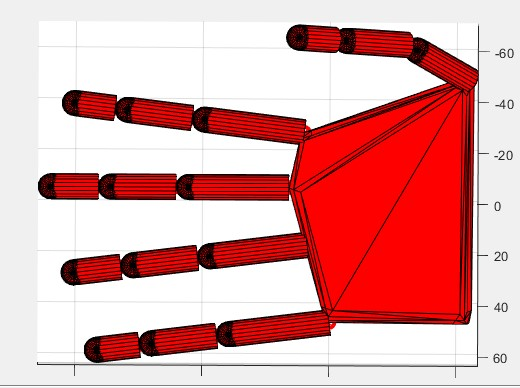
\includegraphics[width=0.4\textwidth]{syngrasp_model.jpg}\quad
	}
	\hfill
%     \subcaption{a}
%\end{minipage}%
%\qquad
%\begin{minipage}{0.05in}%
%\end{minipage}%
%\begin{minipage}{1.2in}%
	\subfloat[]{
      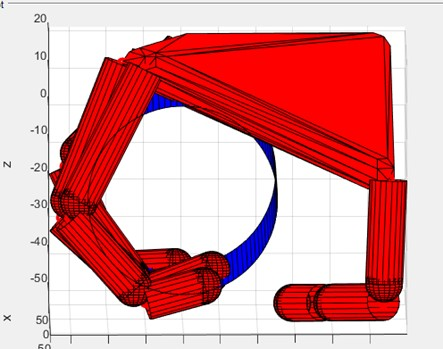
\includegraphics[width=0.4\textwidth]{syngrasp_grip_top}}
	\hfill\null
%     \subcaption{b}
%\end{minipage}%

\caption{By matching the finger dimensions and rotation frames, a SynGrasp model of the Robonaut 2 hand was defined (a).  SynGrasp uses a kinematics solver to generate grasps such as those shown in (b). }%
\label{fig:models}%
\end{figure} 

The first step is to determine the finger angles for grasps of cylinders of varying diameter using SynGrasp to build an initial model for grasping.  The chosen diameters for grasped objects were 2.54 cm, 3.81 cm, 5.08 cm, and 7.62 cm.  The internal contact model in SynGrasp was used to design the grip.  This performed better than traditional inverse kinematic models because it allowed contact with multiple points on the hand rather than only a single point-of-interest on the end-effector.  The key features such as the number of DoFs, finger length, joint rotation frames, and actuation scheme were matched.  Some areas where the modeling program could not match the actual R2 hand were the compliance of the fingers and the size of the palm.  The Robonaut hand contains 18 movable DoFs but only 12 controllable DoFs.  The thumb is fully controllable along every DoF and contains two DoFs at the basilar joint with independent controls for angle at the proximal phalanx and distal phalanx.  The index and middle fingers have 2 rotation DoFs at the metacarpophalangeal joint (MCP), pitch and yaw.  The proximal (PIP) and distal (DIP) interphalangeal joints are underactuated such that they move at matching angles.  The ring and little fingers only take a single input value that controls pitch in all three joints (MCP, PIP, and DIP).  These two fingers have no yawing DoF at the MCP.  The SynGrasp model was provided a synergy matrix to reflect this scheme and grips were designed to include these constraints. 

%TODO: Add figure of R2 hand back in here to show DoF

\subsection{Testing Method} 
A simple testing method was used to validate the models, as well as perform the final experiments to determine grasp efficacy. A cylindrical object was placed on the table, touching R2's open palm. All fingers were fully extended in the starting position.  The object's placement along the palm was varied from near the base of the fingers to the base of the thumb. This allowed testing of uncertainty in position that will be present when the object must be localized. Then, the robot was commanded to close its hand based on the synergy values, lift the object, rotate the object upside down, return it to straight, and finally, release it back on the table. This set of motions demonstrates a firm grasp on the object through a large motion of the robot. 

\begin{figure}[]
  \centering
  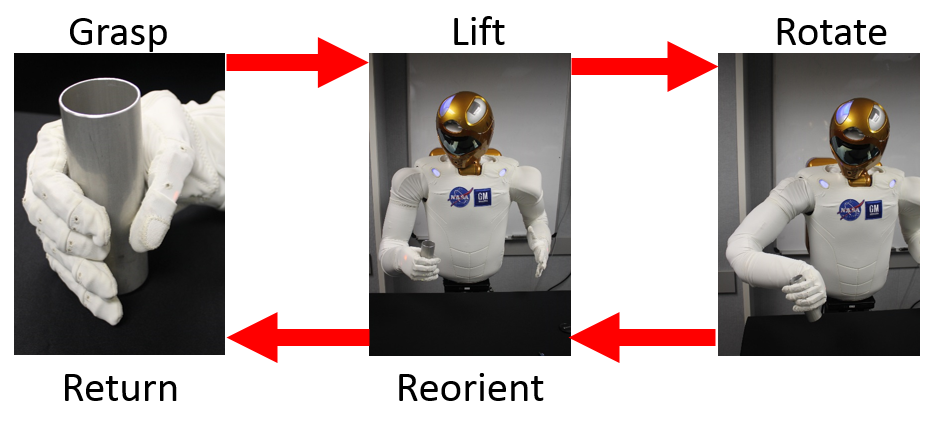
\includegraphics[width=\linewidth]{manipulation}
  \caption{Manipulation action taken by R2 to determine successful grasps}
  \label{testing}
\end{figure}

\subsection{Model Refinement and Synergy Development}
The models were validated by commanding R2's hand to close around a cylindrical piece of aluminum exactly equal to our modeled diameter using the values dictated by SynGrasp. The grasps were tested and refined using the previously mentioned test method and the model discrepancies were accounted for. These discrepancies are discussed in detail in Section \ref{discussion}. Once the final values from testing were established, the results from each cylinder diameter for each finger were plotted and a polynomial fit to the data was carried out. The fits were calculated so that the maximum error for each data point was 4 degrees.   The maximum order used was three, however, many of the joints required lower orders. The resulting relationships were relatively simple which intuitively makes sense, as the object gets larger, the hand opens more. The thumb is the only digit which changed orientations substantially as the diameters got larger as it has more DoF to move into a suitable position. The graph of the thumb joint angle fits are shown in Fig. \ref{thumb_fits}.

\begin{figure}[!b]
  \centering
  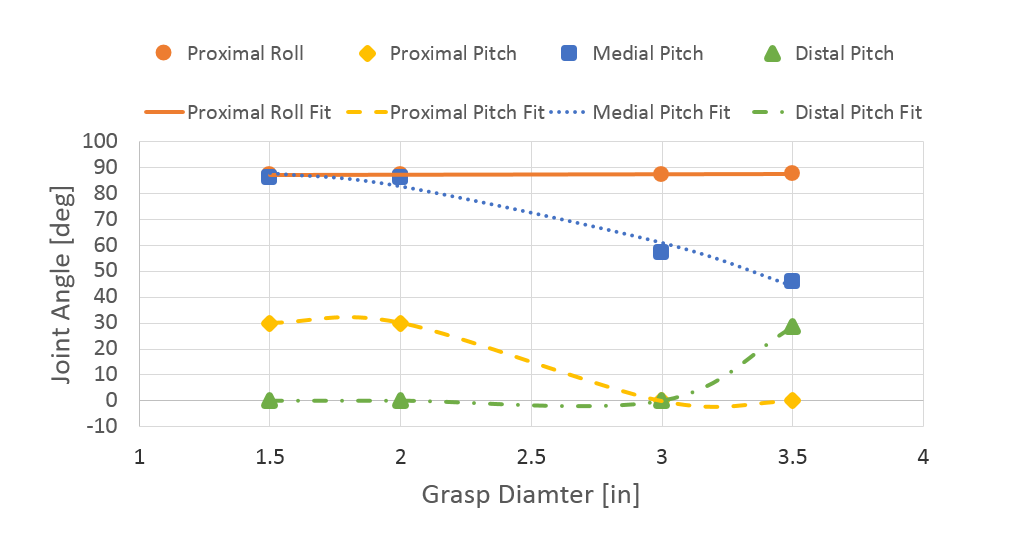
\includegraphics[width=1.08\linewidth]{Thumb_Fits_2}
  \caption{Thumb joint angles when grasping cylinders of varying diameter.  The curve fit shows interpolation between collected data points.}
  \label{thumb_fits} 
\end{figure}


\begin{figure*}[!b]
  \centering
  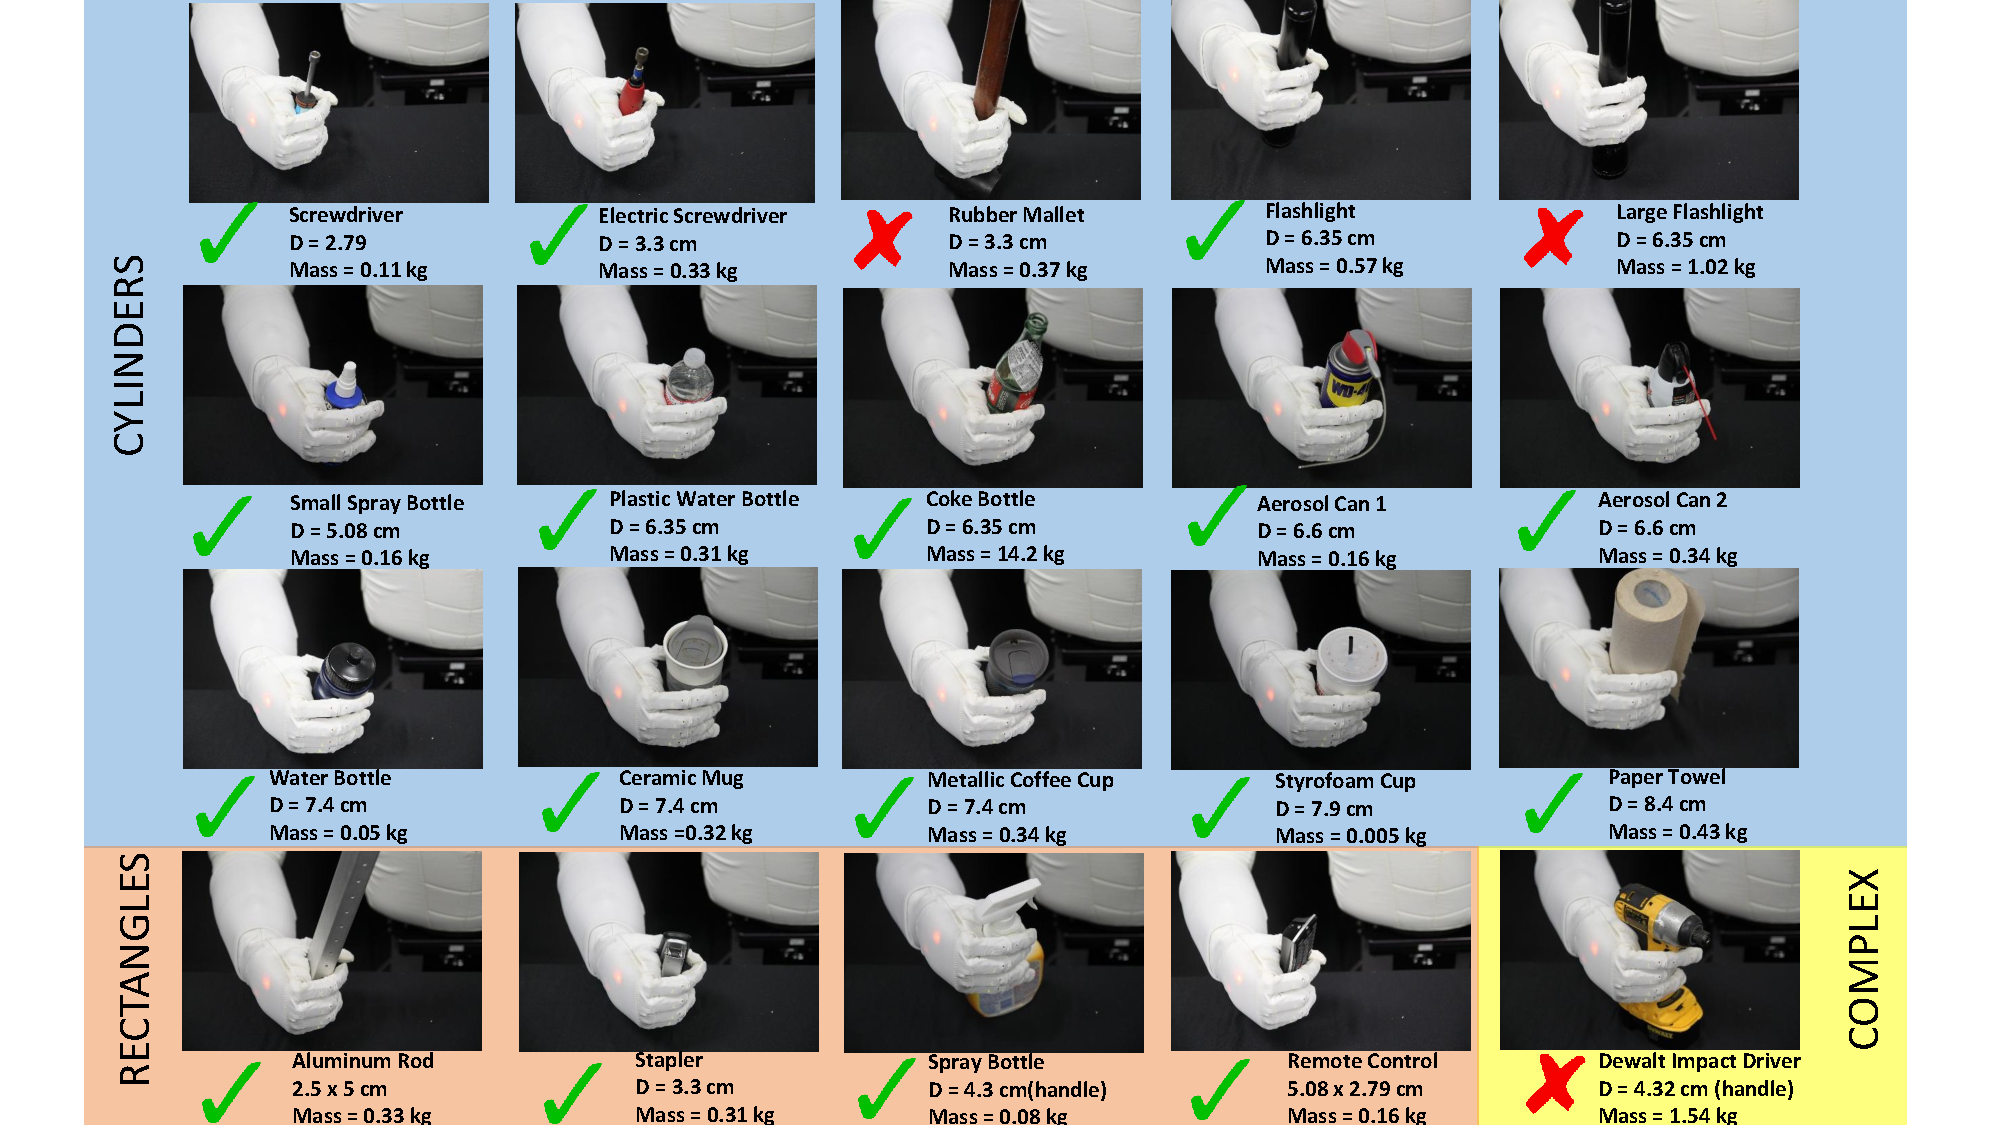
\includegraphics[width=1.08\linewidth]{Objects3.pdf}
  \caption{Results from cylindrical synergy testing using the developed curve fits.  The blue field contrains the pure cylindrical objects.  The orange contains rectangular prisms, and the yellow contains the only complex geometry object, the drill}
  \label{objects} 
\end{figure*}

\section{RESULTS}
\label{results}

REWRITTEN
After model validation on the robot and subsequent adjustments, the robot was able to manipulate 13 of 15 cylindrical objects in the experiment using the single synergy commanding structure. In addition, five non-cylindrical objects were tested, four of which were nearly square rectangular prisms, and one drill. All four rectangular prism objects were successfully grasped which demonstrated the applicability of this synergy to more than pure cylinders. The drill was not successfully grasped showing an example of the case where this method is not applicable.  The list of these objects as well as their success can be viewed in Fig. \ref{objects}. Of the 20 objects manipulated, 17 were manipulated with no issues, 1 slipped in the grip, and 2 were dropped outright. 
REWRITTEN 

\paragraph{}
\section{Discussion}
\label{discussion}

\subsection{SynGrasp Model Validation}

Before the final testing and validation of the system, the SynGrasp model needed to be updated and validated. The SynGrasp model provided a very useful method to determine a starting point for grasp refinement, however, the SynGrasp model remains an idealized model of the robot hand. Many aspects could not be accurately modelled and had to be adjusted through the model validation process, as discussed below. Future additions to the software to allow more realistic actuation could include friction models and more control over the geometry of the hand, as R2's palm is larger than the model allowed. Going forward, SynGrasp is useful for other synergy types such as pinch grasp which has contact forces only in the fingers and does not require use of the palm. 

\begin{figure}[!b]
\centering
\null\hfill
  %\begin{minipage}{2in}
	\subfloat[]{
     	 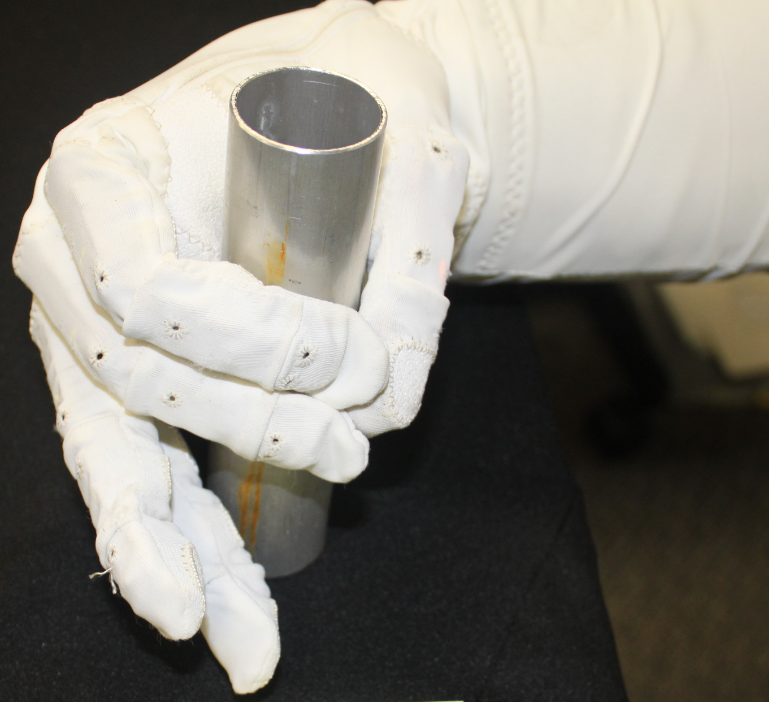
\includegraphics[width=0.45\textwidth]{pinky_out_crop}}\quad
	\hfill
%      \subcaption{a}
 % \end{minipage}%
 % \begin{minipage}{2in}
	\subfloat[]{
      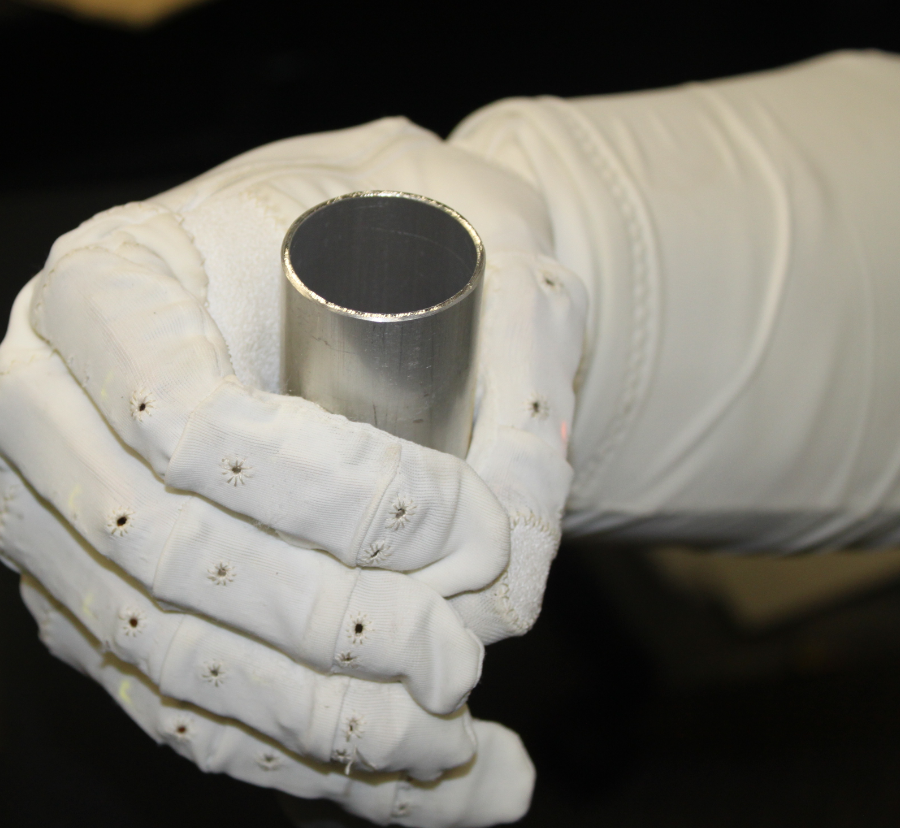
\includegraphics[width=0.45\textwidth]{pinky_in_crop}}
	\hfill\null
 %     \subcaption{b}
  %\end{minipage}
  \caption{Initial (a) and final (b) joint angles for ring and little fingers. The initial round of testing following SynGrasp model generation resulted in no contact in the ring and little fingers.  This result in due to tendon friction in the actual system that reduced the closure angle to a lower value than commanded.}%
\label{pinkymodels}%
\end{figure}

The SynGrasp model assumes the friction among multiple joints actuated with a single tendon is equal, allowing all of the joints to move in unison. However, in practice this is not the case. On the R2 hand, especially on the ring and little fingers, the first joint will move exclusively until it comes into contact with the object, then the next joints will begin to actuate. This resulted in poor finger placement for the ring and little fingers on initial model validation and the closing values had to be increased to obtain a firm grip using those fingers. The result of this can be seen in Fig. \ref{pinkymodels}

In addition, due to a redundant DoF, the 4 DoF thumb has many possible locations in which it could contact the cylinder in SynGrasp which caused the thumb location choice to perform poorly for larger objects near 7.62 cm diameter. Primarily, the thumb would roll too close to the palm, giving a point contact on the thumb pad for larger diameters rather than a wrap around the cylinder. The thumb position was adjusted via testing. The index and middle finger generated by SynGrasp were able to be used with no modifications, demonstrating the usefulness of the initial model in testing and validation. 

A result from the grasping tests was that cylinders near 10 cm were grasped by the robot in a pinch grasp fashion due to the size, so a future pinch grasp model could incorporate larger objects. Also, the geometric synergy method was unable to handle the complex geometry of the drill, which demonstrates that while the synergy concept is useful, it is not directly applicable to all cases and gives an indication of the usefulness of individually actuated joints. Typical manipulation of this tool has the index finger extended, allowing the other fingers to wrap underneath using the synergy-based cylinder grasp values. This could be achieved with a second synergy in combination with the cylinder synergy that weights the extension of the index finger. The combination of these two synergies could create the Dewalt drill grasp and actuation motions in the same framework. This is a concept the authors are leaving for future work. 

\subsection{Grasp Success Discussion}
Once the model was validated, the final testing of the method could be performed. Of the objects selected and tested, 15 could be considered pure cylinders. Of these cylinders, the only one not successfully manipulated at all was the large flashlight. This object slid out of the robot's grasp as it was manipulated. A qualitative evaluation of the grasp suggested the fingers were in an appropriate position. The flashlight was the heaviest object manipulated by the robot (1 kg) and the friction that the robot could apply through the normal force and the glove material was inadequate to manipulate it. The authors believe this is not achievable by the robot regardless of the method of grasp determination. In addition, the robot did not maintain a firm grasp on the hammer. The hammer shank diameter is at the small end of the range that the robot is able to grasp even with a full hand close position due the kinematics of the hand joints and the friction of the glove. The hammer slid in the grasp, but was not dropped. In practice, R2 would be able to manipulate this object to a new location. R2 maintained solid control of the object for all the other cylinders. 

Four prismatic objects were tested to understand the model applicability outside of a pure cylinder. The robot succeeded in manipulating each of these four objects. This suggests that this grasp abstracts to more than cylinders, instead, it could be considered a power grasp synergy, further generalizing the theory. 

Finally, the tested synergy was unable to grasp the Dewalt impact driver. As the robot closed its hand, the index finger caught on the trigger, not allowing the hand to fully wrap around the handle. Upon the rotation action, the Dewalt was dropped. This shows that while the synergy concept is useful, it is not directly applicable to all cases and gives an indication of the usefulness of individually actuated joints. 

Through the testing, the synergy model proposed successfully manipulated all of the cylindrical objects presented in the experiment, demonstrating the usefulness of the concept in practice. The testing also highlighted the further abstraction of the grasp for a cylinder synergy to a power grasp synergy through the manipulation of the prismatic objects. Finally, it was demonstrated that while this synergy is useful for cylinders, additional hand DoFs are still necessary for complex manipulations like that of a drill.

%\subsection{Ease of Use}

%Through this work, the authors conjecture that while previous approaches have sufficiently modeled the hand motions similar to a human, there has been no framework for modeling grasp motions intuitive to a robot user. Santello's work exposed the usefulness of decomposing hand motions into synergies to allow for control on a lower DoF, however, this results in a different control problem to combine non-intuitive motions. Other works use online planning and an accurate object model to determine the appropriate grasp which creates the need for very accurate models or sensors as well as online computational time. The system proposed creates a simple and intuitive model for grasping. Once generated, this model requires effectively no online computation and can be executed with a single, easily understood, user input.

\subsection{Applicability and Future Work}
RE-ADDED
The approach demonstrated in this work shows a useful method of grasping objects commonly manipulated through a power grasp. There is a simple logical step to then apply these methods to determine the synergies for other types of grasp such as a pinch grasp or ball grasp, and effectively change the Cutkosky grasps from single shapes, to sets of relationships. However, to truly do human type manipulation, the individually commanded DoF must remain as shown with the Dewalt drill manipulation. This type of manipulation could be captured in this framework via an additional synergy focused on the position of the index finger. These simple additions could allow individual finger actions that are still intuitive to program to be added to the overall hand motions that have been demonstrated to work. 
RE-ADDED
 
\section{CONCLUSIONS}

The authors demonstrated a novel concept to incorporate the synergy framework developed in neuroscience and analyzed in practice  into an intuitive commanding strategy for a high DoF robot hand on Robonaut 2. The creation of a synergy based on the diameter of a cylindrical object allowed cylinders of varying sizes to be effectively grasped via a single command input. The results of this test suggest that this concept could be used to quickly broaden the library of objects the robot can manipulate from a small, specialized set, into a nearly infinite library of manipulatable cylinders. 

\bibliographystyle{splncs}

\bibliography{BibFile}


\end{document}
